% Created 2017-02-11 Sat 01:57
% Intended LaTeX compiler: pdflatex
\documentclass[a4paper,11pt]{article}
\usepackage[utf8]{inputenc}
\usepackage[T1]{fontenc}
\usepackage{graphicx}
\usepackage{grffile}
\usepackage{longtable}
\usepackage{wrapfig}
\usepackage{rotating}
\usepackage[normalem]{ulem}
\usepackage{amsmath}
\usepackage{textcomp}
\usepackage{amssymb}
\usepackage{capt-of}
\usepackage{hyperref}
\usepackage[margin=1.2in]{geometry}
\usepackage{setspace}
\onehalfspacing
\usepackage{parskip}
\usepackage{amsthm}
\usepackage{amsmath}
\usepackage{mathtools}
\usepackage{hyperref}
\usepackage{graphicx}
\usepackage{tabularx}
\usepackage{booktabs}
\hypersetup{colorlinks,citecolor=black,filecolor=black,linkcolor=black,urlcolor=black}
\newtheorem{definition}{Definition}
\newtheorem{theorem}{Theorem}
\newcommand{\dx}{\mathrm{d}}
\newcommand{\var}{\mathrm{Var}}
\newcommand{\cov}{\mathrm{Cov}}
\newcommand{\corr}{\mathrm{Corr}}
\newcommand{\pr}{\mathrm{Pr}}
\newcommand{\rarrowd}[1]{\xrightarrow{\text{ \textit #1 }}}
\DeclareMathOperator*{\plim}{plim}
\newcommand{\plimn}{\plim_{n \rightarrow \infty}}
\setcounter{secnumdepth}{2}
\author{Zheng Tian}
\date{}
\title{Lecture 1: Economic Questions and Data}
\hypersetup{
 pdfauthor={Zheng Tian},
 pdftitle={Lecture 1: Economic Questions and Data},
 pdfkeywords={},
 pdfsubject={},
 pdfcreator={Emacs 25.1.1 (Org mode 9.0.3)}, 
 pdflang={English}}
\begin{document}

\maketitle
\setcounter{tocdepth}{1}
\tableofcontents


\section{What is Econometrics?}
\label{sec:org3ee4e63}

\subsection{Definition of Econometrics}
\label{sec:org3cb51c5}

Econometricians may give you very different answers for the question
of \emph{What is Econometrics}. The following answers are all right from
their respective point of views:
\begin{itemize}
\item econometrics is the science of testing economic theories;
\item it is the set of tools used to forecasting future values
of economic variables;
\item it is the process of fitting mathematical economic model
to real-world data;
\item it is the science and art of using historical data to make
quantitative policy recommendations in government and business.
\end{itemize}

Stock and Watson (2015) define Econometrics as
\begin{quote}
At a broad level, econometrics is the science and art of using
economic theory and statistical techniques to analyze economic
data.
\end{quote}



\subsection{Science or art?}
\label{sec:orgcc77cf9}

Let us dissect the above definition a little bit. First, why is
econometrics the science AND art?

\begin{itemize}
\item Econometrics is a science because it essentially complies with the
principle of \textbf{falsifiability} of scientific research, as Karl Popper
defined. Figure \ref{fig:org810b5e4} show a typical reasoning cycle
of a scientific research.\footnote{Source of Figure \ref{fig:org810b5e4}: Martyn Shuttleworth (Sep
21, 2008). Falsifiability. Retrieved Feb 10, 2017 from Explorable.com:
\url{https://explorable.com/falsifiability}.}

\begin{figure}[htbp]
\centering
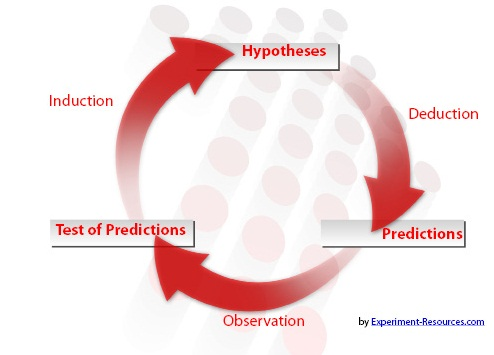
\includegraphics[width=0.6\textwidth]{figure/reasoning-cycle-research.jpg}
\caption{\label{fig:org810b5e4}
A reasoning cycle of scientific research}
\end{figure}

Econometricians propose a hypothesis based on either existing economic
theories or their own economic reasoning, and then collect data to
test the hypothesis that can be rejected or fail to be rejected. Even
though an economic theory is not rejected by one set of data at a
time period, it can be very likely to be rejected using another set of
data at another time period. Then, a new theory or hypothesis will
be brought up.

\item Econometrics is an art because the data are usually incomplete and
unobserved to validate a hypothesis, so we need to use human
creativity to reach a balance between scientific rigor and realistic
approximation.
\end{itemize}

The following quote captures the dual nature of econometrics as both
science and art:
\begin{quote}
Econometrics is alchemy since econometricians can create nearly any
result desired, but it is also science because econometricians also
know how to reject and avoid spurious models. -- Hansen (1996)
\end{quote}


\subsection{Economic theory, statistics, and data}
\label{sec:orgac0f946}

A complete process of econometric research inevitably consists of three
components: economic theory, statistical techniques, and economic
data. When we have a research question, we first need to find or
formulate an economic theory that can be either a formal mathematical
model or a logical economic reasoning. Guided with this economic
theory, we build an econometric model to characterize the relationship
between various variables involved in the theory. Then we collect data
to measure these variables, and use statistical techniques to estimate
the model and test hypotheses that are raised from the theory.

\begin{figure}[htbp]
\centering
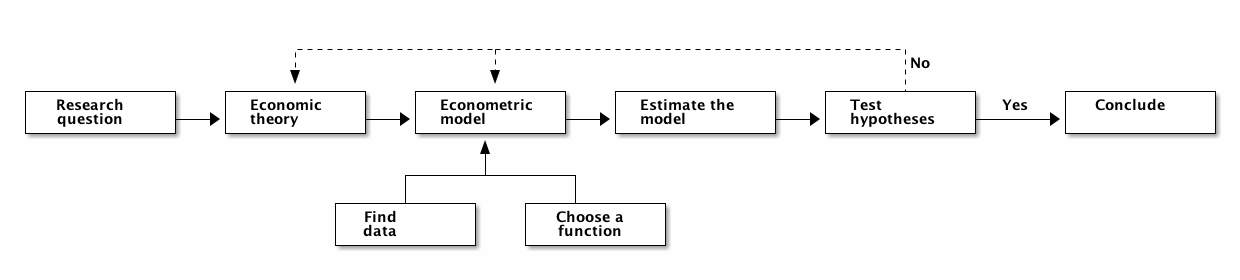
\includegraphics[width=1.0\textwidth]{figure/econometric_workflow.png}
\caption{A workflow of econometric research}
\end{figure}

Let's look at a real example to get a first impression of what is
econometrics.


\section{Economic Questions We Examine}
\label{sec:org0593572}

\subsection{Four practical questions}
\label{sec:org09f75b3}

\begin{description}
\item[{Question 1}] does reducing class size improve elementary school education?

\item[{Question 2}] is there racial discrimination in the market for home loan?

\item[{Question 3}] how much do cigarette taxes reduce smoking?

\item[{Question 4}] what will the rate of inflation be next year?
\end{description}


\subsection{How does an econometrician formulate such questions?}
\label{sec:org5b05299}

Ideally, an econometrician would design his/her econometric modeling
by the following steps

\begin{enumerate}
\item Establish a theoretical model to qualitatively describe how X could
cause Y, holding other factors constant. From the theoretical
model, put forward some hypotheses to validate the theory.
\item Find actual data to measure the variables in the theory
\item Set up an empirical model to test the theoretical model, using
available data.
\item Choose a suitable estimation method to estimate the empirical model.
\item Perform some hypothesis tests and model specification test to
validate the estimation results.
\item Based on the estimation and test results, determine whether the theory
is internally and externally valid.
\end{enumerate}


\section{Causal Effects and Idealized Experiments}
\label{sec:org5c01698}

The success of an econometric analysis relies on whether the causal
effects between X and Y can be accurately identified, excluding the
influences of other factors.

\subsection{Randomized controlled experiment}
\label{sec:org3b943c0}

\subsubsection*{Controlled experiment}
\label{sec:orgbbdadb3}

Control group (no treatment) versus treatment group (with treatment)

\subsubsection*{Randomized experiment}
\label{sec:org6c458a7}
the treamtment is assigned randomly

\subsubsection*{Advantages and disadvantages}
\label{sec:org68a14b0}

\begin{description}
\item[{Advantages}] eliminate the possibility of a systematic relationship that could
blur the causal effects of the treatment

\item[{Disadvantages}] it is difficult to implement, especially for social
science
\end{description}


\section{Data Sources and Types}
\label{sec:orgc3aaa37}
\subsection{{\bfseries\sffamily TODO} Experimental versus observational data}
\label{sec:orgbbf3f79}

\subsection{Cross-sectional data}
\label{sec:orgab41fc0}

\begin{itemize}
\item heights of all 30 students in a class

\item total population of each province in China in 2014
\end{itemize}

\subsection{Time series data}
\label{sec:org2862fae}

\begin{itemize}
\item stock price of Company A by hour over the last month

\item consumer price index of China by month from 1990 to 2014
\end{itemize}

\subsection{Panel data}
\label{sec:org47a24b8}

\begin{itemize}
\item annual wage of a fixed group of respondents in a survey conducted by
a statistic agency in 1990, 1995, 2000, 2005, and 2010

\item GDP per capita of each country in Asia from 1990 to 2014
\end{itemize}
\end{document}